% Copyright 2004 by Till Tantau <tantau@users.sourceforge.net>.
%
% In principle, this file can be redistributed and/or modified under
% the terms of the GNU Public License, version 2.
%
% However, this file is supposed to be a template to be modified
% for your own needs. For this reason, if you use this file as a
% template and not specifically distribute it as part of a another
% package/program, I grant the extra permission to freely copy and
% modify this file as you see fit and even to delete this copyright
% notice. 
  
\documentclass[spanish,pdf]{beamer}
\usepackage{etex}
\usepackage[spanish,es-tabla]{babel}
\usepackage[utf8]{inputenc}
\usepackage{amsmath,amssymb,latexsym}
% Doe's not play well with memoir
\usepackage{subfigure}
%\usepackage{pifont}
%\usepackage[linktocpage=true]{hyperref}
\usepackage{algorithm}
%\usepackage[noend]{algpseudocode}
\usepackage{booktabs}
\usepackage{wrapfig}
\usepackage{xspace}
\usepackage{multirow}
\usepackage{adjustbox}
\usepackage[figuresleft]{rotating}
\usepackage{rotfloat}
\usepackage[final]{fixme}
\usepackage{multicol}
\usepackage{smartdiagram}
\usepackage{tikz}
\usetikzlibrary{automata,petri,positioning,shapes,snakes,arrows,backgrounds,babel}
\tikzstyle{tplace}=[circle,draw,inner sep=1.8mm]
\usepackage{amsthm}
% Encabezado "lindo"
% Memoir y fancyhdr definen ambos esto. Pero lo definen igual, así que no hay problema
% Fuente: http://tex.stackexchange.com/questions/37868/fancyhdr-and-memoir
\let\footruleskip\undefined
\usepackage{caption}
\usepackage{fancyhdr}
% Saca los espacios adicionales de las listas tipo itemize
%\usepackage{enumitem}
%\setlist{nolistsep}
%\usepackage{hypcap}
% Para armar código bonito
%\usepackage{minted}
%\usemintedstyle{bw}
\usepackage{xcolor}
\usepackage[framemethod=default]{mdframed}
\definecolor{bg}{rgb}{0.95,0.95,0.95}
\mdfdefinestyle{codebox}{backgroundcolor=bg,skipabove=10,linewidth=0}
\usepackage[most]{tcolorbox}

\usepackage{czt}
\usepackage{algpseudocode}
\setbeamerfont{block body}{size=\scriptsize}
%\usepackage{xcolor}
%
%\usepackage[most]{tcolorbox}

%\usetheme{Madrid}
%\usetheme{Antibes}
%\usetheme{Copenhagen}
\usetheme{Warsaw}
\mode<presentation>{} 

\newcommand{\til}{\widetilde}
%\newcommand{\inv}{\overline}
\newcommand{\bsl}{\backslash}
\newcommand{\loor}{\vee}
\newcommand{\loand}{\wedge}
\newcommand{\xor}{\oplus}
\newcommand{\subs}{\subset}
\newcommand{\subse}{\subseteq}
\newcommand{\sups}{\supset}
\newcommand{\supse}{\supseteq}
\newcommand{\ror}{\vdash}
\newcommand{\Ror}{\models}
\newcommand{\rar}{\rightarrow}
\newcommand{\mrar}{$\rightarrow$}
\newcommand{\Rar}{\Rightarrow}
\newcommand{\URar}[1]{\stackrel{#1}{\Rar }}
\newcommand{\Urar}[1]{\stackrel{#1}{\rar }}
\newcommand{\ULRar}[1]{\stackrel{#1}{\Longrightarrow }}
\newcommand{\Ulrar}[1]{\stackrel{#1}{\longrightarrow }}
\newcommand{\paral}{\parallel}
\newcommand{\emptys}{\emptyset}
\newcommand{\mult}{\times}
\newcommand{\verx}{\vspace{12pt}}
\newcommand{\niz}{\vspace{10pt}}
\newcommand{\eproof}{\hspace{\fill} $\Box $}
\newcommand{\ediamon}{\hspace{\fill} $\Diamond $}


% Alex's predicates

\newcommand{\ins}{\mbox{\tt in}}
\newcommand{\IN}{\mbox{\tt IN}}
\newcommand{\out}{\mbox{\tt out}}
\newcommand{\OUT}{\mbox{\tt OUT}}
\newcommand{\INOUT}{\mbox{\tt IN\_OUT}}
\newcommand{\exit}{\mbox{\tt exit}}
\newcommand{\EXIT}{\mbox{\tt EXIT}}
\newcommand{\enter}{\mbox{\tt enter}}
\newcommand{\nocross}{\mbox{\tt nocross}}
\newcommand{\ENTER}{\mbox{\tt ENTER}}
\newcommand{\inexit}{\mbox{\tt in\_exit}}
\newcommand{\inenter}{\mbox{\tt in\_enter}}
\newcommand{\enterexit}{\mbox{\tt enter\_exit}}
\newcommand{\exitenter}{\mbox{\tt enter\_exit}}
\newcommand{\outexit}{\mbox{\tt out\_exit}}
\newcommand{\outenter}{\mbox{\tt out\_enter}}
\newcommand{\genet}{\mbox{\tt Genet}}
\newcommand{\petrify}{\mbox{\tt petrify}}
\newcommand{\mlc}{\mbox{\tt MLC}}

\newtheorem{exam}{Example}[section]
\newtheorem{prop}{Proposition}[section]
\newenvironment{condition}[1]{\noindent{\bf Condition #1.} \em}{\rm \\}

\newcommand{\bop}{\noindent{\bf Proof: }}
\newcommand{\eop}{$\square$ \\}
%\newenvironment{proof}{\bop}{\eop}
%\newtheorem{lemma}{Lemma}[section]
%\newtheorem{theorem}{Theorem}[section]
%\newtheorem{corollary}{Corollary}[section]
%\newtheorem{proposition}{Proposition}[section]
%\newtheorem{property}{Property}[section]
%\newtheorem{definition}{Definition}[section]
%\newtheorem{problem}{Problem}[section]
%\newtheorem{procedure}{Procedure}[section]
%\newtheorem{restriction}{Restriction}[section]
%\newtheorem{algorithm}{Algorithm}
\def\acs/{{\sf ACS}}
\def\ets/{{\sf ETS}}
\def\ec/{{\sf EC}}
\def\eec/{{\sf EEC}}
\def\ects/{{\sf ECTS}}
\def\eects/{{\sf EECTS}}
\def\nts/{{\sf NTS}}
\def\gnts/{{\sf GNTS}}
\def\eer/{{\sf EER}}
\def\esr/{{\sf ESR}}
\def\en/{{\sf EN}}
\def\ger/{{\sf GER}}
\def\er/{{\sf ER}}
\def\sr/{{\sf SR}}
\def\gsr/{{\sf GSR}}
\def\bacs/{{\sf BACS}}
\def\ts/{{\sf TS}}
\def\lts/{{\sf LTS}}
\def\alts/{{\sf ALTS}}
\def\std/{{\sf STD}}
\def\cd/{{\sf CD}}
\def\alc/{{\sf ALC}}
\def\id/{{\sf ID}}
\def\pd/{{\sf PD}}

\def\stg/{{\sf STG}}
\def\cln/{{\sf CLN}}
\def\clstg/{{\sf CL-STG}}
\def\btm/{{Binary Trace Model}}
\def\tm/{{Trace Model}}

\newcommand{\pn}{\textsf{PN}}
\newcommand{\rg}{\textsf{RG}}
\newcommand{\rs}{\textsf{RS}}
\newcommand{\prs}{\textsf{PRS}}
\newcommand{\pl}{\textsf{PL}}

\newcommand{\mg}{\mbox{\textsf{MG}}}       % Marked graph
\def\dr/{{Distributive}}
\def\drone/{{Distributive-1}}
\def\drtwo/{{Distributive-2}}
\def\op/{{Output-persistent}}
\def\sm/{{\sf SM}}
\def\bull{\vrule height .9ex width .8ex depth -.1ex }
%\def\trans#1{\stackrel{#1}{\rightarrow}}
\def\dquote#1{``#1''}
\def\trans#1{[#1>}
\def\etrans#1{E(#1)}
\def\vect#1#2{$#1_1,\ldots,#1_{#2}$}
\def\assign#1#2{\mbox{$#1 \leftarrow #2$}}
\def\tild{{\verb+~+}}
\def\pred#1{\,^\bullet #1}
\def\succ#1{#1^\bullet}
\def\prereg#1{\,^\circ #1}
\def\postreg#1{#1^\circ}
\def\prepostreg#1{\,^\circ #1^\circ}
\def\endofproof{\hspace{\fill} $\Box $}


\def\grad#1#2{\Delta_{#1}(#2)}
\def\pow#1{#1^\diamond}
\def\enabling#1{^\star#1}
\def\rzero{\mbox{\bf 0}}
\def\rone{\mbox{\bf 1}}
\def\rk{\mbox{\bf K}}
\def\REG{{\mathcal R}}
\def\TOP{\sqcap}
\def\sup{\mbox{\em supp}}
\def\topk{\top}
%  Nomenclature for Petri nets, STGs, etc.

\newcommand{\reachm}[1]{[#1\rangle}             % reachable markings
\newcommand{\firing}[3]{\mbox{$#1\Ulrar{#2} #3$}} % Transition firing
\newcommand{\altfiring}[3]{#1[#2\rangle #3}        % Alternative transition firing
\newcommand{\preset}[1]{\mbox{$^\bullet#1$}}             % Preset
\newcommand{\postset}[1]{\mbox{$#1^\bullet$}}            % Postset
\newcommand{\pmlog}{\ensuremath{{\mathcal L}}}        % Log
\newcommand{\pmlogp}{\ensuremath{{\mathcal L}}\textsuperscript{+}}        % Positive Log
\newcommand{\pmlogn}{\ensuremath{{\mathcal L}}\textsubscript{-}}        % Negative Log
\newcommand{\ph}{\ensuremath{{\mathcal P}}}          % Polyhedron
\newcommand{\parikh}[1]{\ensuremath{\Pi(#1)}}    % Set of Parikh vectors

% Natural numbers
%\newcommand{\nat}{\ensuremath{\mathbb{N}}}

\newcommand\bench[2][]{%
\if\relax\detokenize{#1}\relax%
\textsc{#2}\else \textsc{#2}\hspace{0.3pt}{\footnotesize(}#1{\footnotesize)}\fi\@\xspace}

\newcommand\pnsimp  {\textsc{PNsimpl}\@\xspace}
\newcommand\pachtool  {\textsc{PacH}\@\xspace}
\newcommand\qhulltool  {\textsc{Qhull}\@\xspace}

\newcommand{\model}{\mathcal{M}}
\newcommand{\sys}{\mathcal{S}}
\newcommand{\Language} {\mathcal{L}}


\newcommand{\nlgtext}[1] {``\emph{#1}''}
\newcommand{\nlgfun}[1] {\texttt{#1}}
\newcommand{\reglaverb}[2]{\item #1 \\ \hspace*{0.56cm} $\rightarrow$ #2}
% fix para 
\renewcommand*\Call[2]{\textproc{#1}(#2)}

% Equations commands
% Begin equation no numbered
\newcommand{\bnnequation}{\begin{equation*}}
% Begin equation mode
\newcommand{\bequation}{\begin{equation*}}
% Begin equation mode with label
\newcommand{\bequationl}[1]{\begin{equation}\label{eq:#1}}
% End equation mode
\newcommand{\eequation}{\end{equation*}}
% End labeled equation mode
\newcommand{\eequationl}{\end{equation}}
% End equation no numbered
\newcommand{\ennequation}{\end{equation*}}

%Math symbols
\newcommand{\sigmap}{\ensuremath{\sigma}\textsuperscript{+}}        % Positive Sigma
\newcommand{\sigman}{\ensuremath{\sigma}\textsuperscript{-}}        % Negative Sigma
\newcommand{\eventstar}{\ensuremath{T}\textsuperscript{*}}        % Event Set T*

% Condensed table
\newcommand\newrow{\\[-1.5pt]}
\newcommand\tvdots{\multicolumn{1}{c}{$\vdots$}}

% Scale input
\newcommand{\scaledinput}[2]{\scalebox{#1}{\input{#2}}}


\definecolor{mygreen}{rgb}{0,0.5,0}
% Algoritmos en español
\floatname{algorithm}{Algoritmo}
%\renewcommand{\listalgorithmname}{Lista de algoritmos}
\renewcommand{\algorithmicrequire}{\textbf{Entrada:}}
\renewcommand{\algorithmicensure}{\textbf{Salida:}}


\addtobeamertemplate{navigation symbols}{}{%
    \usebeamerfont{footline}%
    \usebeamercolor[fg]{footline}%
    \hspace{1em}%
    \insertframenumber/\inserttotalframenumber
}

\AtBeginSection[]
{
  \begin{frame}<beamer>
    \frametitle{Contenidos}
    \tableofcontents[currentsection]
  \end{frame}
}
  
%\title{Generación de lenguaje natural a partir de clases de prueba del \textit{test template framework}}
  
% A subtitle is optional and this may be deleted
%\subtitle{Optional Subtitle}
  
%\author{F.~Author\inst{1} \and S.~Another\inst{2}}
% - Give the names in the same order as the appear in the paper.
% - Use the \inst{?} command only if the authors have different
%   affiliation.
  
%\institute[Universities of Somewhere and Elsewhere] % (optional, but mostly needed)
%{
%  \inst{1}%
%  Department of Computer Science\\
%  University of Somewhere
%  \and
%  \inst{2}%
%  Department of Theoretical Philosophy\\
%  University of Elsewhere}
% - Use the \inst command only if there are several affiliations.
% - Keep it simple, no one is interested in your street address.
  
%\date{Conference Name, 2013}
% - Either use conference name or its abbreviation.
% - Not really informative to the audience, more for people (including
%   yourself) who are reading the slides online
  
\subject{Computer Science}
% This is only inserted into the PDF information catalog. Can be left
% out. 
  
% If you have a file called "university-logo-filename.xxx", where xxx
% is a graphic format that can be processed by latex or pdflatex,
% resp., then you can add a logo as follows:
  
\pgfdeclareimage[height=0.5cm]{university-logo}{../img/unr.png}
\logo{\pgfuseimage{university-logo}}
  
% Delete this, if you do not want the table of contents to pop up at
% the beginning of each subsection:
%\AtBeginSubsection[]
%{
%    \begin{frame}<beamer>{Contenidos}
%        \tableofcontents[currentsection,currentsubsection]
%    \end{frame}
%}
  
% Let's get started
\begin{document}
  
\title[Gen. y simp. de especificaciones de procesos de producción]{Generación y simplificación automática de especificaciones de procesos de producción}
\institute[FCEIA - UNR]{
  Departamento de Ciencias de la Computación\\
  Facultad de Ciencias Exactas, Ingeniería y Agrimensura\\
  Universidad Nacional de Rosario
}
\author[Lucio Nardelli]{\begin{tabular}{r@{ }l} 
  Autor:      & Lucio Nardelli \\[1ex]
  Director:   & Hernán Ponce de León\\
  \end{tabular}}
\date{Junio, 2016}
  
\begin{frame}
  \titlepage
\end{frame}
  
%\begin{frame}{Outline}
  %\tableofcontents
  % You might wish to add the option [pausesections]
%\end{frame}
  
\section{Introducción}
  
\begin{frame}{Motivación}{}
    \begin{itemize}
      \setlength\itemsep{0.4cm}
      \item<2-> Hoy en día existe un acceso masivo a sistemas informáticos.
      \item<3-> Esto genera inmensas cantidades de información.
      \item<4-> Dependencia total de estos sistemas, es esencial mantenerlos eficientes y seguros.
      \item<5-> ¿Cómo se puede asegurar esto?
      \item<6-> Utilizaremos métodos de representación formal.
    \end{itemize}
\end{frame}

\begin{frame}{Motivación}{Modelos formales}
  \vspace*{-0.5cm}
  \begin{minipage}[c][0.4\textheight][c]{\linewidth}
    Utilizar un modelo gráfico, que sea de fácil de entender
    pero formal para que se permita un análisis del sistema subyacente.
  \end{minipage}
  \begin{columns}
    \column{0.25\textwidth}
  \pause 
      \begin{minipage}[c][0.3\textheight][c]{\linewidth}
        \centering
        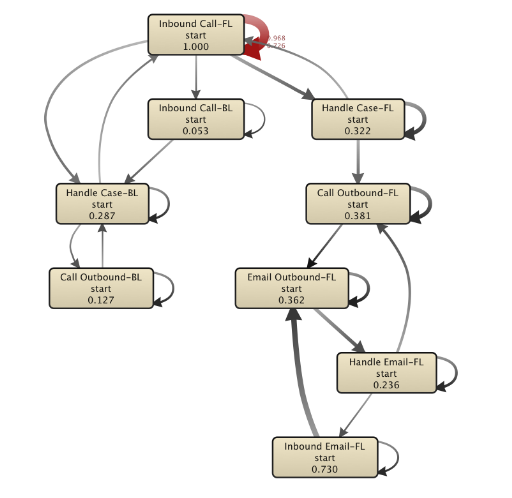
\includegraphics[width=1.2\linewidth]{img/ejemplo1.png}
      \end{minipage}
    \column{0.45\textwidth}
  \pause 
      \begin{minipage}[c][0.3\textheight][c]{\linewidth}
        \centering
        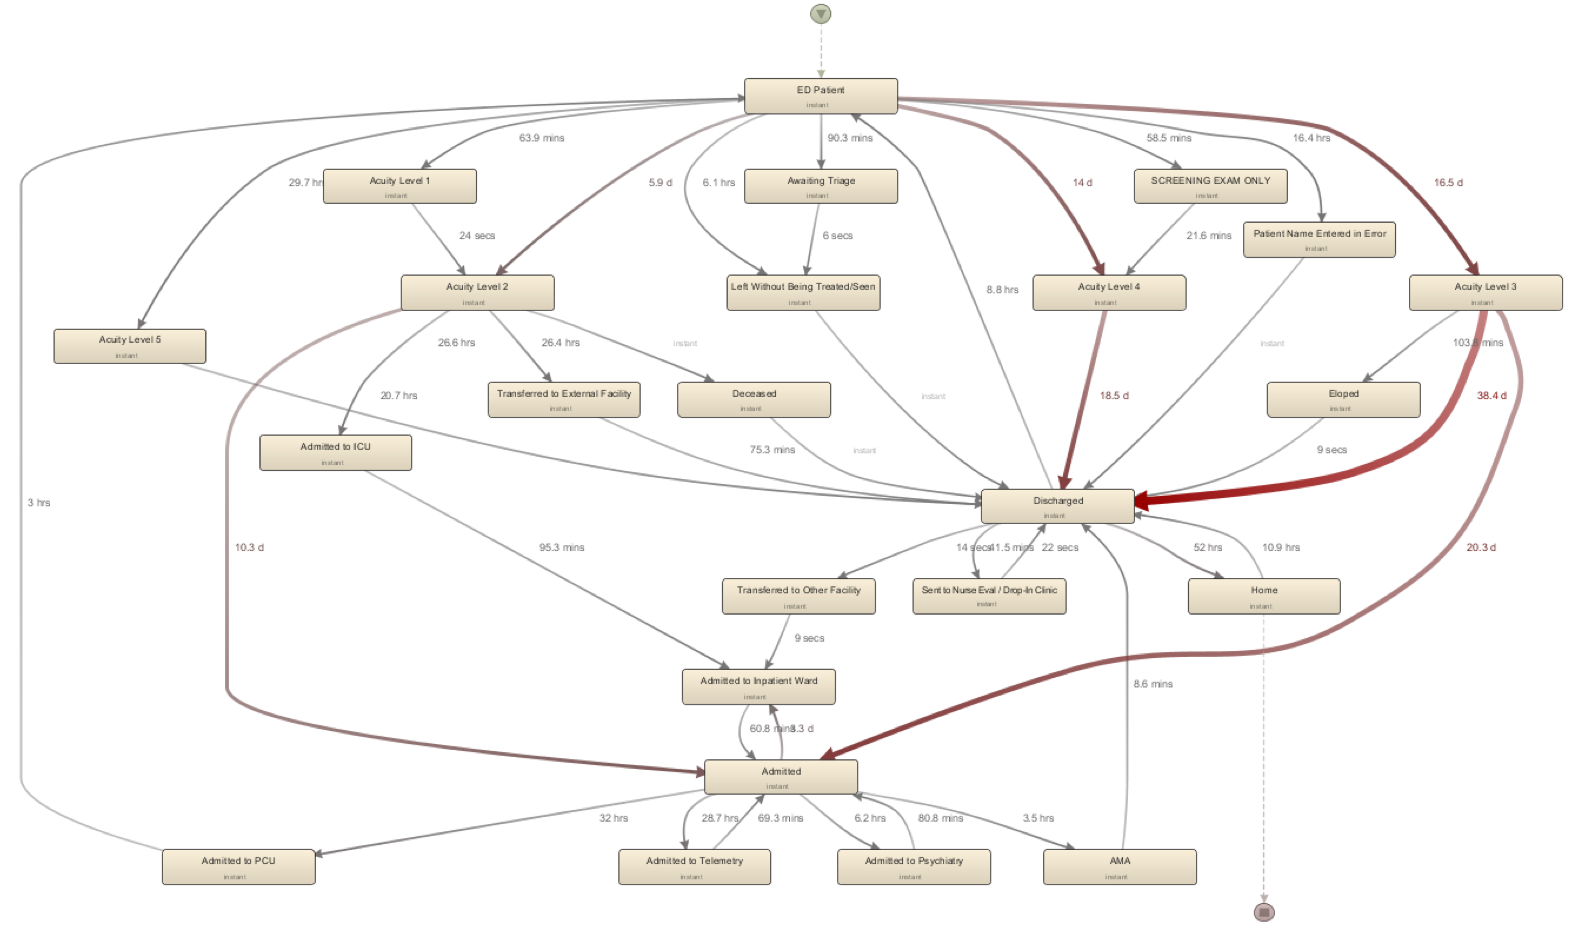
\includegraphics[width=1.2\linewidth]{img/ejemplo2.png}
      \end{minipage}
    \column{0.3\textwidth}
  \pause 
      \begin{minipage}[c][0.05\textheight][c]{\linewidth}
        \centering
        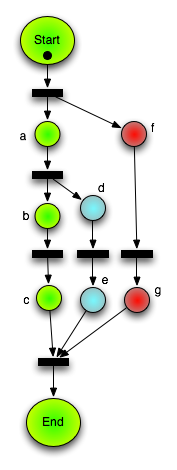
\includegraphics[width=0.5\linewidth]{img/ejemplo3.png}
      \end{minipage}
  \end{columns}
  \vspace*{-0.5cm}
  \pause 
  \begin{minipage}[c][0.4\textheight][c]{\linewidth}
    El problema es que estos modelos formales, ¡rara vez existen!
  \end{minipage}
\end{frame}

\begin{frame}{Motivación}{Descubrimiento de procesos}
    \begin{itemize}
      \setlength\itemsep{0.4cm}
      \item<2-> Para obtener el modelo recurrimos al \textit{descubrimiento de procesos}.
      \item<3-> Es una técnica de aprendizaje automatizado.
      \item<4-> Transforma un registro de acciones de un sistema en un modelo formal.
    \end{itemize}
    \tikzset{every shadow/.style={fill=none,shadow scale=0}}
    \smartdiagramset{border color=none,
      set color list={white!100!white,red!50!black,black!90!white,blue!50!green},
      back arrow disabled=true}
    \vspace*{0.5cm}
    \pause[5]
    \smartdiagram[flow diagram:horizontal]{Sistema,Info en crudo,ACME - Black Box, Modelo Formal}
                
                %los \textit{logs de eventos} de un sistema.
%    \pause[4]
%        Pero...¿qué es un log de eventos de un sistema?
%    \begin{itemize}
%      \item<5-> Un log de eventos consiste de un archivo donde se describe un conjunto de trazas de un sistema; 
%          es decir se lleva registro ordenado de las acciones relevantes que ocurren durante la ejecución de un sistema.
%    \end{itemize}
\end{frame}

\begin{frame}{Motivación}{Minería de procesos gráficamente}
  \centering
  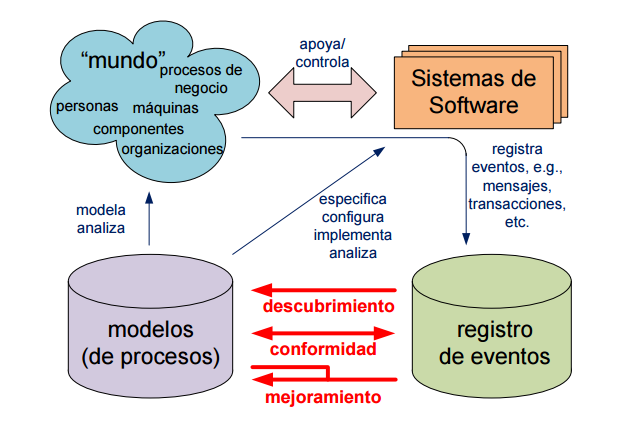
\includegraphics[width=0.95\linewidth]{img/pmcycle.png}
\end{frame}

\begin{frame}{Motivación}{Mejora de modelos}
  \begin{itemize}
    \item<1-> Problema con las técnicas de descubrimiento: modelos \textit{spaghetti}.
  \end{itemize}
  \pause[2]
  \only<2>{
    \centering
    
\includegraphics[width=0.5\linewidth]{img/lady_and_tramp.jpg}

    Los spaghetti pueden ser una muy buena idea para una cena romántica, 
    pero no son una buena idea para un modelo formal...
  }
  \begin{columns}
    \column{0.45\textwidth}
      \pause[3]
      \centering
      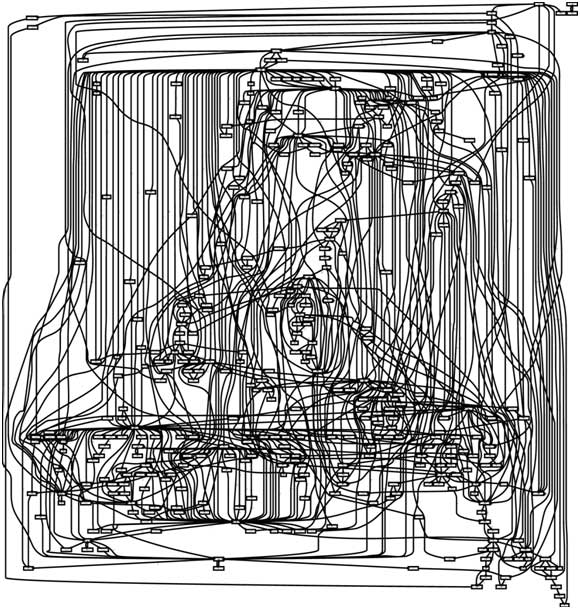
\includegraphics[width=0.8\linewidth]{img/spaghetti_model_2.jpg}
    \column{0.45\textwidth}
      \pause[4]
      \centering
      
\includegraphics[width=0.5\linewidth]{img/homero_grita.jpg}

      ¿Quién podría entender algo de un modelo como ese?
  \end{columns}
\end{frame}

\begin{frame}{Motivación}{Mejora de modelos}
   \begin{itemize}
      \setlength\itemsep{0.4cm}
      \item<1-> Para mejorarlos se aplican técnicas de \textit{mejora de modelos}
      \item<2-> Puede lograrse considerando las trazas más frecuentes o bien información de comportamientos que \textit{no} deben ocurrir.
    \end{itemize}
%    \pause[4]
%        Pero...¿qué es la información negativa?
%    \begin{itemize}
%      \item<5-> La información negativa consiste en un conjunto de trazas que el sistema no debe realizar nunca.
%    \end{itemize}
\end{frame}

\begin{frame}{Motivación}{Objetivo general}
  \begin{itemize}
    \setlength\itemsep{0.4cm}

    \item<1-> Obtener un modelo formal de manera automática a partir de los logs de eventos de un sistema.
    
    \item<2-> Optimizar el modelo obtenido mediante técnicas de mejora de modelos para obtener un modelo que
          resulte simple.
    
    \item<3-> Automatizar los puntos anteriores.

  \end{itemize}
\end{frame}

\section{Nociones preliminares}

\begin{frame}{Redes de Petri}{Ejemplo de la evolución de una red de Petri}
  \begin{columns}
    \column{0.3\textwidth}
      \only<1>{\usetikzlibrary{arrows,shapes,automata,petri,positioning}

\tikzset{
    placeyellow/.style={
        circle,
        thick,
        draw=yellow!75,
        fill=red!20,
        minimum size=6mm,
    },
    place/.style={
        circle,
        thick,
        draw=blue!75,
        fill=blue!20,
        minimum size=6mm,
    },
    transitionH/.style={
        rectangle,
        thick,
        fill=black,
        minimum width=8mm,
        inner ysep=2pt
    },
    transitionV/.style={
        rectangle,
        thick,
        fill=black,
        minimum height=8mm,
        inner xsep=2pt
    },
    transitionVgreen/.style={
        rectangle,
        thick,
        fill=green!25,
        minimum height=8mm,
        inner xsep=2pt
    },
    transitionVred/.style={
        rectangle,
        thick,
        fill=red!75,
        minimum height=8mm,
        inner xsep=2pt
    },
    transitionVdgreen/.style={
        rectangle,
        thick,
        fill=green!75,
        minimum height=8mm,
        inner xsep=2pt
    }
}


\begin{tikzpicture}[node distance=0.5cm and 1cm,>=stealth',bend angle=45,auto]
    \node [place,tokens=3,label=above:$P_1$] (p1) {};
    \node [transitionV,label=below:$T_1$] (t1) [right= of p1] {}
        edge[pre] node[swap]{\scriptsize 3}  (p1);
    \node [place,tokens=1,label=above:$P_2$] (p2) [above right=of t1] {}
        edge[pre]   (t1);
    \node [place,tokens=2,label=above:$P_3$] (p3) [below right=of t1] {}
        edge[pre]   (t1);
    \node [transitionV,label=below:$T_2$] (t2) [above right=of p3] {}
        edge[pre] node[swap]{\scriptsize 2} (p2)
        edge[pre]   (p3)
        edge[post,out=50,in=70,looseness=2,overlay]  node[swap]{\scriptsize 4} (p1);
\end{tikzpicture}


}
      \only<2>{\usetikzlibrary{arrows,shapes,automata,petri,positioning}

\tikzset{
    placeyellow/.style={
        circle,
        thick,
        draw=yellow!75,
        fill=red!20,
        minimum size=6mm,
    },
    place/.style={
        circle,
        thick,
        draw=blue!75,
        fill=blue!20,
        minimum size=6mm,
    },
    transitionH/.style={
        rectangle,
        thick,
        fill=black,
        minimum width=8mm,
        inner ysep=2pt
    },
    transitionV/.style={
        rectangle,
        thick,
        fill=black,
        minimum height=8mm,
        inner xsep=2pt
    },
    transitionVgreen/.style={
        rectangle,
        thick,
        fill=green!25,
        minimum height=8mm,
        inner xsep=2pt
    },
    transitionVred/.style={
        rectangle,
        thick,
        fill=red!75,
        minimum height=8mm,
        inner xsep=2pt
    },
    transitionVdgreen/.style={
        rectangle,
        thick,
        fill=green!75,
        minimum height=8mm,
        inner xsep=2pt
    }
}


\begin{tikzpicture}[node distance=0.5cm and 1cm,>=stealth',bend angle=45,auto]
    \node [place,tokens=1,label=above:$P_1$] (p1) {};
    \node [transitionV,label=below:$T_1$] (t1) [right= of p1] {}
        edge[pre]   (p1);
    \node [place,tokens=1,label=above:$P_2$] (p2) [above right=of t1] {}
        edge[pre]   (t1);
    \node [place,tokens=2,label=above:$P_3$] (p3) [below right=of t1] {}
        edge[pre]   (t1);
    \node [transitionVred,label=below:$T_2$] (t2) [above right=of p3] {}
        edge[pre] node[swap]{\scriptsize 2} (p2)
        edge[pre]   (p3)
        edge[post,out=50,in=70,looseness=2,overlay]  (p1);
\end{tikzpicture}


}
      \only<3>{\usetikzlibrary{arrows,shapes,automata,petri,positioning}

\tikzset{
    placeyellow/.style={
        circle,
        thick,
        draw=yellow!75,
        fill=yellow!20,
        minimum size=6mm,
    },
    place/.style={
        circle,
        thick,
        draw=blue!75,
        fill=blue!20,
        minimum size=6mm,
    },
    transitionH/.style={
        rectangle,
        thick,
        fill=black,
        minimum width=8mm,
        inner ysep=2pt
    },
    transitionV/.style={
        rectangle,
        thick,
        fill=black,
        minimum height=8mm,
        inner xsep=2pt
    },
    transitionVgreen/.style={
        rectangle,
        thick,
        fill=green!25,
        minimum height=8mm,
        inner xsep=2pt
    },
    transitionVred/.style={
        rectangle,
        thick,
        fill=red!75,
        minimum height=8mm,
        inner xsep=2pt
    },
    transitionVdgreen/.style={
        rectangle,
        thick,
        fill=green!75,
        minimum height=8mm,
        inner xsep=2pt
    }
}


\begin{tikzpicture}[node distance=0.5cm and 1cm,>=stealth',bend angle=45,auto]
    \node [place,tokens=3,label=above:$P_1$] (p1) {};
    \node [transitionVdgreen,label=below:$T_1$] (t1) [right= of p1] {}
        edge[pre] node[swap]{\scriptsize 3}  (p1);
    \node [place,tokens=1,label=above:$P_2$] (p2) [above right=of t1] {}
        edge[pre]   (t1);
    \node [place,tokens=2,label=above:$P_3$] (p3) [below right=of t1] {}
        edge[pre]   (t1);
    \node [transitionVred,label=below:$T_2$] (t2) [above right=of p3] {}
        edge[pre] node[swap]{\scriptsize 2} (p2)
        edge[pre]   (p3)
        edge[post,out=50,in=70,looseness=2,overlay]  node[swap]{\scriptsize 4} (p1);
\end{tikzpicture}


}
      \only<4>{\usetikzlibrary{arrows,shapes,automata,petri,positioning}

\tikzset{
    placeyellow/.style={
        circle,
        thick,
        draw=yellow!75,
        fill=yellow!20,
        minimum size=6mm,
    },
    place/.style={
        circle,
        thick,
        draw=blue!75,
        fill=blue!20,
        minimum size=6mm,
    },
    transitionH/.style={
        rectangle,
        thick,
        fill=black,
        minimum width=8mm,
        inner ysep=2pt
    },
    transitionV/.style={
        rectangle,
        thick,
        fill=black,
        minimum height=8mm,
        inner xsep=2pt
    },
    transitionVgreen/.style={
        rectangle,
        thick,
        fill=green!25,
        minimum height=8mm,
        inner xsep=2pt
    },
    transitionVred/.style={
        rectangle,
        thick,
        fill=red!75,
        minimum height=8mm,
        inner xsep=2pt
    },
    transitionVdgreen/.style={
        rectangle,
        thick,
        fill=green!75,
        minimum height=8mm,
        inner xsep=2pt
    }
}


\begin{tikzpicture}[node distance=0.5cm and 1cm,>=stealth',bend angle=45,auto]
    \node [placeyellow,label=above:$P_1$] (p1) {};
    \node [transitionVdgreen,label=below:$T_1$] (t1) [right= of p1] {}
        edge[pre] node[swap]{\scriptsize 3}  (p1);
    \node [place,tokens=1,label=above:$P_2$] (p2) [above right=of t1] {}
        edge[pre]   (t1);
    \node [place,tokens=2,label=above:$P_3$] (p3) [below right=of t1] {}
        edge[pre]   (t1);
    \node [transitionVred,label=below:$T_2$] (t2) [above right=of p3] {}
        edge[pre] node[swap]{\scriptsize 2} (p2)
        edge[pre]   (p3)
        edge[post,out=50,in=70,looseness=2,overlay]  node[swap]{\scriptsize 4} (p1);
\end{tikzpicture}


}
      \only<5>{\usetikzlibrary{arrows,shapes,automata,petri,positioning}

\tikzset{
    placeyellow/.style={
        circle,
        thick,
        draw=yellow!75,
        fill=yellow!20,
        minimum size=6mm,
    },
    place/.style={
        circle,
        thick,
        draw=blue!75,
        fill=blue!20,
        minimum size=6mm,
    },
    transitionH/.style={
        rectangle,
        thick,
        fill=black,
        minimum width=8mm,
        inner ysep=2pt
    },
    transitionV/.style={
        rectangle,
        thick,
        fill=black,
        minimum height=8mm,
        inner xsep=2pt
    },
    transitionVgreen/.style={
        rectangle,
        thick,
        fill=green!60,
        minimum height=8mm,
        inner xsep=2pt
    },
    transitionVred/.style={
        rectangle,
        thick,
        fill=red!75,
        minimum height=8mm,
        inner xsep=2pt
    },
    transitionVdgreen/.style={
        rectangle,
        thick,
        fill=green!75,
        minimum height=8mm,
        inner xsep=2pt
    }
}


\begin{tikzpicture}[node distance=0.5cm and 1cm,>=stealth',bend angle=45,auto]
    \node [place,label=above:$P_1$] (p1) {};
    \node [transitionVdgreen,label=below:$T_1$] (t1) [right= of p1] {}
        edge[pre] node[swap]{\scriptsize 3}  (p1);
    \node [placeyellow,tokens=2,label=above:$P_2$] (p2) [above right=of t1] {}
        edge[pre]   (t1);
    \node [placeyellow,tokens=3,label=above:$P_3$] (p3) [below right=of t1] {}
        edge[pre]   (t1);
    \node [transitionVred,label=below:$T_2$] (t2) [above right=of p3] {}
        edge[pre] node[swap]{\scriptsize 2} (p2)
        edge[pre]   (p3)
        edge[post,out=50,in=70,looseness=2,overlay]  node[swap]{\scriptsize 4} (p1);
\end{tikzpicture}


}
      \only<6>{\usetikzlibrary{arrows,shapes,automata,petri,positioning}

\tikzset{
    placered/.style={
        circle,
        thick,
        draw=red!75,
        fill=red!20,
        minimum size=6mm,
    },
    place/.style={
        circle,
        thick,
        draw=blue!75,
        fill=blue!20,
        minimum size=6mm,
    },
    transitionH/.style={
        rectangle,
        thick,
        fill=black,
        minimum width=8mm,
        inner ysep=2pt
    },
    transitionV/.style={
        rectangle,
        thick,
        fill=black,
        minimum height=8mm,
        inner xsep=2pt
    },
    transitionVgreen/.style={
        rectangle,
        thick,
        fill=green!60,
        minimum height=8mm,
        inner xsep=2pt
    },
    transitionVred/.style={
        rectangle,
        thick,
        fill=red!75,
        minimum height=8mm,
        inner xsep=2pt
    },
    transitionVdgreen/.style={
        rectangle,
        thick,
        fill=green!75,
        minimum height=8mm,
        inner xsep=2pt
    }
}


\begin{tikzpicture}[node distance=0.5cm and 1cm,>=stealth',bend angle=45,auto]
    \node [place,label=above:$P_1$] (p1) {};
    \node [transitionVred,label=below:$T_1$] (t1) [right= of p1] {}
        edge[pre] node[swap]{\scriptsize 3}  (p1);
    \node [place,tokens=2,label=above:$P_2$] (p2) [above right=of t1] {}
        edge[pre]   (t1);
    \node [place,tokens=3,label=above:$P_3$] (p3) [below right=of t1] {}
        edge[pre]   (t1);
    \node [transitionV,label=below:$T_2$] (t2) [above right=of p3] {}
        edge[pre] node[swap]{\scriptsize 2} (p2)
        edge[pre]   (p3)
        edge[post,out=50,in=70,looseness=2,overlay]  node[swap]{\scriptsize 4} (p1);
\end{tikzpicture}


}
      \only<7>{\usetikzlibrary{arrows,shapes,automata,petri,positioning}

\tikzset{
    placered/.style={
        circle,
        thick,
        draw=red!75,
        fill=red!20,
        minimum size=6mm,
    },
    place/.style={
        circle,
        thick,
        draw=blue!75,
        fill=blue!20,
        minimum size=6mm,
    },
    transitionH/.style={
        rectangle,
        thick,
        fill=black,
        minimum width=8mm,
        inner ysep=2pt
    },
    transitionV/.style={
        rectangle,
        thick,
        fill=black,
        minimum height=8mm,
        inner xsep=2pt
    },
    transitionVgreen/.style={
        rectangle,
        thick,
        fill=green!60,
        minimum height=8mm,
        inner xsep=2pt
    },
    transitionVred/.style={
        rectangle,
        thick,
        fill=red!75,
        minimum height=8mm,
        inner xsep=2pt
    },
    transitionVdgreen/.style={
        rectangle,
        thick,
        fill=green!75,
        minimum height=8mm,
        inner xsep=2pt
    }
}


\begin{tikzpicture}[node distance=0.5cm and 1cm,>=stealth',bend angle=45,auto]
    \node [place,label=above:$P_1$] (p1) {};
    \node [transitionVred,label=below:$T_1$] (t1) [right= of p1] {}
        edge[pre] node[swap]{\scriptsize 3}  (p1);
    \node [place,tokens=2,label=above:$P_2$] (p2) [above right=of t1] {}
        edge[pre]   (t1);
    \node [place,tokens=3,label=above:$P_3$] (p3) [below right=of t1] {}
        edge[pre]   (t1);
    \node [transitionVdgreen,label=below:$T_2$] (t2) [above right=of p3] {}
        edge[pre] node[swap]{\scriptsize 2} (p2)
        edge[pre]   (p3)
        edge[post,out=50,in=70,looseness=2,overlay]  node[swap]{\scriptsize 4} (p1);
\end{tikzpicture}


}
      \only<8>{\usetikzlibrary{arrows,shapes,automata,petri,positioning}

\tikzset{
    placeyellow/.style={
        circle,
        thick,
        draw=yellow!75,
        fill=yellow!20,
        minimum size=6mm,
    },
    place/.style={
        circle,
        thick,
        draw=blue!75,
        fill=blue!20,
        minimum size=6mm,
    },
    transitionH/.style={
        rectangle,
        thick,
        fill=black,
        minimum width=8mm,
        inner ysep=2pt
    },
    transitionV/.style={
        rectangle,
        thick,
        fill=black,
        minimum height=8mm,
        inner xsep=2pt
    },
    transitionVgreen/.style={
        rectangle,
        thick,
        fill=green!60,
        minimum height=8mm,
        inner xsep=2pt
    },
    transitionVred/.style={
        rectangle,
        thick,
        fill=red!75,
        minimum height=8mm,
        inner xsep=2pt
    },
    transitionVdgreen/.style={
        rectangle,
        thick,
        fill=green!75,
        minimum height=8mm,
        inner xsep=2pt
    }
}


\begin{tikzpicture}[node distance=0.5cm and 1cm,>=stealth',bend angle=45,auto]
    \node [place,label=above:$P_1$] (p1) {};
    \node [transitionVred,label=below:$T_1$] (t1) [right= of p1] {}
        edge[pre] node[swap]{\scriptsize 3}  (p1);
    \node [placeyellow,tokens=0,label=above:$P_2$] (p2) [above right=of t1] {}
        edge[pre]   (t1);
    \node [placeyellow,tokens=2,label=above:$P_3$] (p3) [below right=of t1] {}
        edge[pre]   (t1);
    \node [transitionVdgreen,label=below:$T_2$] (t2) [above right=of p3] {}
        edge[pre] node[swap]{\scriptsize 2} (p2)
        edge[pre]   (p3)
        edge[post,out=50,in=70,looseness=2,overlay]  node[swap]{\scriptsize 4} (p1);
\end{tikzpicture}


}
      \only<9>{\usetikzlibrary{arrows,shapes,automata,petri,positioning}

\tikzset{
    placeyellow/.style={
        circle,
        thick,
        draw=yellow!75,
        fill=yellow!20,
        minimum size=6mm,
    },
    place/.style={
        circle,
        thick,
        draw=blue!75,
        fill=blue!20,
        minimum size=6mm,
    },
    transitionH/.style={
        rectangle,
        thick,
        fill=black,
        minimum width=8mm,
        inner ysep=2pt
    },
    transitionV/.style={
        rectangle,
        thick,
        fill=black,
        minimum height=8mm,
        inner xsep=2pt
    },
    transitionVgreen/.style={
        rectangle,
        thick,
        fill=green!60,
        minimum height=8mm,
        inner xsep=2pt
    },
    transitionVred/.style={
        rectangle,
        thick,
        fill=red!75,
        minimum height=8mm,
        inner xsep=2pt
    },
    transitionVdgreen/.style={
        rectangle,
        thick,
        fill=green!75,
        minimum height=8mm,
        inner xsep=2pt
    }
}


\begin{tikzpicture}[node distance=0.5cm and 1cm,>=stealth',bend angle=45,auto]
    \node [placeyellow,tokens=4,label=above:$P_1$] (p1) {};
    \node [transitionV,label=below:$T_1$] (t1) [right= of p1] {}
        edge[pre] node[swap]{\scriptsize 3}  (p1);
    \node [place,tokens=0,label=above:$P_2$] (p2) [above right=of t1] {}
        edge[pre]   (t1);
    \node [place,tokens=2,label=above:$P_3$] (p3) [below right=of t1] {}
        edge[pre]   (t1);
    \node [transitionVred,label=below:$T_2$] (t2) [above right=of p3] {}
        edge[pre] node[swap]{\scriptsize 2} (p2)
        edge[pre]   (p3)
        edge[post,out=50,in=70,looseness=2,overlay]  node[swap]{\scriptsize 4} (p1);
\end{tikzpicture}


}
    \column{0.7\textwidth}
      \centering
      % Define box and box title style
\tikzstyle{mybox} = [draw=gray!60, fill=white, thick,
    rectangle, rounded corners, inner ysep=1pt, inner sep=1pt]%, inner sep=10pt, inner ysep=20pt]

\begin{tikzpicture}

% First box
\pause[2]
\node [mybox] (box1){%
  \begin{minipage}{0.25\textwidth}
  \scriptsize
  \bequation
    \begin{array}{l}
        M_0(p_1) = 3\\
        M_0(p_2) = 1\\
        M_0(p_3) = 2\\
    \end{array}
  \eequation
  \end{minipage}
};

\pause[5]
% Second Box, placed with 1cm distance below box1
\node [mybox,below=1cm of box1.south] (box2) {%
  \begin{minipage}[t!]{0.6\textwidth}
  \scriptsize
  \bequation
    \begin{array}{l}
        M_1(p_1) = M_0(p_1)-3 = 0\\
        M_1(p_2) = M_0(p_2)+1 = 2\\
        M_1(p_3) = M_0(p_3)+1 = 3\\
    \end{array}
  \eequation
  \end{minipage}
}
% Draw a connection line between box1 and box2 with the same style like the box:
edge [pre] node[auto,swap] {T1} (box1)
;

\pause[9]
% Third Box, placed with 1cm distance below box2
\node [mybox,below=1cm of box2.south] (box3) {%
  \begin{minipage}[t!]{0.95\textwidth}
  \scriptsize
  \bequation
    \begin{array}{l}
        M_2(p_1) = M_1(p_1)+4 = M_0(p_1)-3+4 = 4\\
        M_2(p_2) = M_1(p_2)-2 = M_0(p_2)+1-2 = 0\\
        M_2(p_3) = M_1(p_2)-1 = M_0(p_3)+1-1 =2\\
    \end{array}
  \eequation

  \end{minipage}
}
% Draw a connection line between box2 and box3 with the same style like the box:
edge [pre] node[auto,swap] {T2} (box2)
;

\end{tikzpicture}
%


  \end{columns}
\end{frame}

\begin{frame}{Redes de Petri}{Evolución de una red de Petri}
    \begin{itemize}
      \setlength\itemsep{0.2cm}
      \item<2-> Los markings pueden definirse de manera incremental como
        \bnnequation
            M'(p) = M(p) - F(p,t) +  F(t,p).
        \ennequation
      \item<3-> Más general, ante una sucesión de eventos:
        \bnnequation
          M(p) = M_0(p) + \sum_{x_i}F(x_i,p)\cdot \widehat\sigma(x_i) - \sum_{y_i}F(p,y_i)\cdot\widehat\sigma(y_i).
        \ennequation
      \item<4-> Utilizando notación matricial, puede definirse para todos los places de una red:
        \bnnequation
          M = M_0 + A \cdot \widehat\sigma.
        \ennequation
  \end{itemize}
\end{frame}

\begin{frame}{Enfoque del trabajo}{}
  \centering
  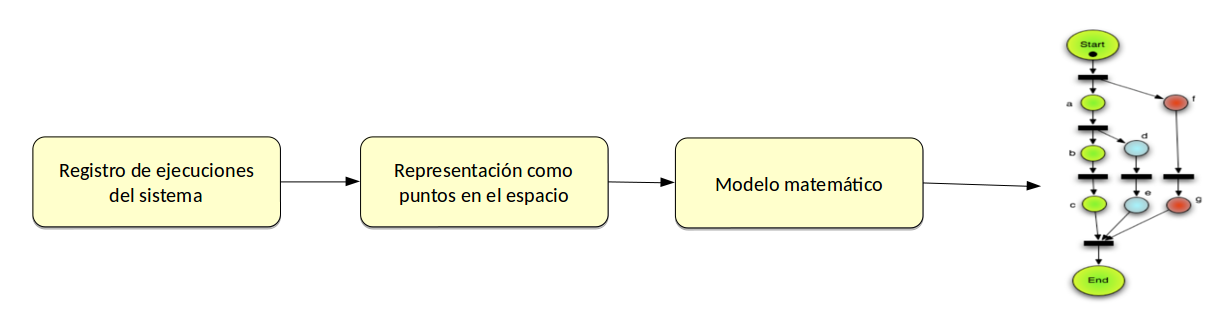
\includegraphics[width=1.0\linewidth]{img/approach_simplificado.png}
  \pause
  \begin{itemize}
    \setlength\itemsep{0.2cm}
    \item El registro de ejecuciones es generado por el sistema en los \textit{logs de eventos}.
    \item La representación como puntos en el espacio corresponde al \textit{conjunto de vectores Parikh} del log.
    %\item El modelo matemático corresponde a un poliedro convexo que contenga el conjunto de vectores Parikh.
  \end{itemize}
\end{frame}

\begin{frame}{De logs y vectores Parikh}{Conceptos}
  \scriptsize
  \begin{itemize}
    \setlength\itemsep{0.1cm}
    \item<1-> Un \textit{log de eventos} es un conjunto de trazas o sucesión ordenada de actividades relevantes de un sistema.

    \item<2-> Dada una traza $\sigma=\sigma_1\cdot\sigma_2\cdot\ldots\cdot\sigma_k$ sobre un alfabeto
        $T=\{t_1,t_2,\dots,t_n\}$, el \textit{vector Parikh} corresponde a la cantidad de ocurrencias
        de cada acción $t_i$ en $\sigma$.
  \end{itemize}

  \pause[3]
   \begin{example}
       Para las trazas $\sigma_1=t_1 \cdot t_2 \cdot t_1 \cdot t_2 \cdot t_1 \cdot t_1 \cdot t_3$ y $\sigma_2=t_4 \cdot t_4$,
       sobre el alfabeto $T=\{t_1,t_2,t_3,t_4\}$ los vectores de Parikh de cada traza vienen dados por las tuplas $(4,1,1,0)$ y $(0,0,0,2)$ respectivamente.
   \end{example}

  \begin{columns}
    \column{0.3\textwidth}
        \pause[5]
        \centering
        
\includegraphics[width=1.2\linewidth]{img/homer-simpson-cooking.jpg}
    \column{0.7\textwidth}
        \pause[4]
        Entonces, teníamos un log de eventos y ahora podemos convertirlo en tuplas de enteros...
  \end{columns}
\end{frame}

\begin{frame}{Enfoque del trabajo}{}
  \centering
  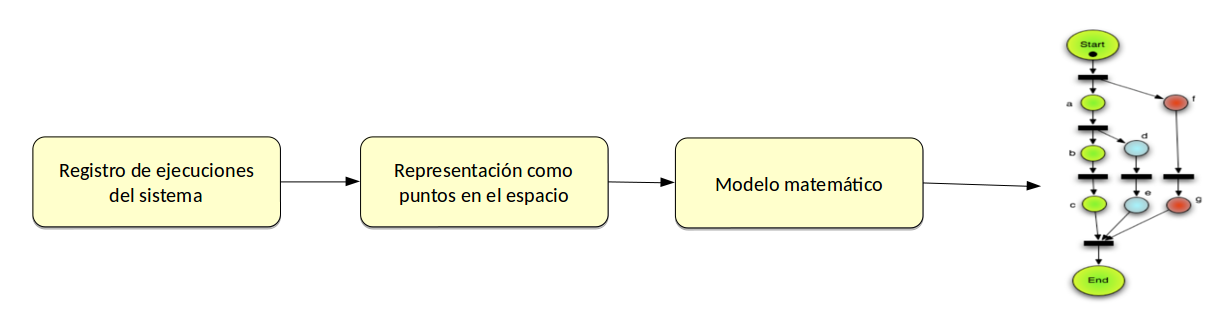
\includegraphics[width=1.0\linewidth]{img/approach_simplificado.png}
  \begin{itemize}
    \setlength\itemsep{0.2cm}
    \item<1-> El registro de ejecuciones es generado por el sistema en los \textit{logs de eventos}.
    \item<1-> La representación como puntos en el espacio corresponde al conjunto de vectores Parikh del log.
    \item<2-> El modelo matemático corresponde a un poliedro convexo que contenga el conjunto de vectores Parikh.
  \end{itemize}
\end{frame}
\begin{frame}{Dominios numéricos abstractos}{Poliedros convexos}
  \begin{columns}

    \column{0.3\textwidth}
      \scaledinput{0.3}{img/polyhedra}

    \column{0.5\textwidth}
      \begin{itemize}
        \scriptsize
        \setlength\itemsep{0.2cm}
        \item<2-> Los \textit{semi-espacios} se representan mediante una inecuación lineal de la forma $a_1x_1 + a_2x_2 + \cdots + a_nx_n \geq b.$
        \item<3-> Un poliedro convexo $\ph$ puede representarse como una intersección de un conjunto de $k$ hiper-espacios
            \bnnequation
                \ph = \{ x \in \mathbb{R}^n ~|~ A\cdot x + b \geq 0\}
            \ennequation
            donde  \mbox{$A \in \mathbb{R}^{k \times n}$} y \mbox{$b\in\mathbb{R}^{k}$}.
      \end{itemize}

  \end{columns}
\end{frame}

\begin{frame}{Descubrimiento de procesos}{¡Juntemos todo!}
  \begin{columns}
    \column{0.6\textwidth}
        \centering
        \scaledinput{0.3}{discovery/walks}
    \column{0.25\textwidth}
        \scaledinput{0.9}{discovery/walks_net1}
    \column{0.25\textwidth}
        \scaledinput{0.9}{discovery/walks_net2}
  \end{columns}
\end{frame}

\section{Desarrollo}

\begin{frame}{Descubrimiento de procesos}{Simplificación}
  \begin{minipage}[c][0.2\textheight][c]{\linewidth}
  \begin{itemize}
      \item<1-> Modelos excesivamente complicados y alejados de la realidad.
      \item<1->Necesidad de simplificar. 
  \end{itemize}
  \end{minipage}
\only<1>{
  \begin{minipage}[c][0.2\textheight][c]{\linewidth}
    $$\begin{array}{rcccccccl}
        120 & + & 64 \cdot x_1 & + & 33  \cdot x_2 & + & -10 \cdot x_3 & \ge & 0 \\
        -40 & + & 14 \cdot x_1 & - & 62 \cdot x_2 & + & 8   \cdot x_3 & \ge & 0 \\
        -83 & + & 20 \cdot x_1 & + & 46  \cdot x_2 & + & 40  \cdot x_3 & \ge & 0 \\
    \end{array}$$
  \end{minipage}
}
\pause[2]
  \begin{minipage}[c][0.2\textheight][c]{\linewidth}
    $$\begin{array}{rcccccccl}
        ??? & + & ??? \cdot x_1 & + & ??? \cdot x_2 & + & ??? \cdot x_3 & \ge & 0 \\
        ??? & + & ??? \cdot x_1 & + & ??? \cdot x_2 & + & ??? \cdot x_3 & \ge & 0 \\
        ??? & + & ??? \cdot x_1 & + & ??? \cdot x_2 & + & ??? \cdot x_3 & \ge & 0 \\
    \end{array}$$
  \end{minipage}
  \begin{itemize}
      \item<3-> Buscamos nuevos coeficientes para el sistema de inecuaciones: 
        \begin{itemize}
            \item Los nuevos coeficientes deben ser más ``simples''.
            \item Cada solución del sistema original tiene que continuar siendo
                una solución del nuevo sistema.
        \end{itemize}
  \end{itemize}
\end{frame}

\begin{frame}{Descubrimiento de procesos}{Simplificación}
\scriptsize
  \begin{minipage}[c][0.3\textheight][c]{\linewidth}
    Dado un modelo de la forma: 
    $$\begin{array}{rcccccccl}
        \alpha_{1,0} & + & \alpha_{1,1} \cdot x_1 & + & \dots & + & \alpha_{1,n} \cdot x_n & \ge & 0 \\
        \alpha_{2,0} & + & \alpha_{2,1} \cdot x_1 & + & \dots & + & \alpha_{2,n} \cdot x_n & \ge & 0 \\
            \ldots & & & & & & \ldots \\
        \alpha_{m,0} & + & \alpha_{m,1} \cdot x_1 & + & \dots & + & \alpha_{m,n} \cdot x_n & \ge & 0
    \end{array}$$
  \end{minipage}

\pause
Se buscan nuevos coeficientes $\beta_{1,0},\beta_{1,1}, \dots, \beta_{m,n}$ tal que:

\bequationl{enc2} \tag{MIN}
    \rvert \beta_{i,j} \lvert\ \leq\ \rvert \alpha_{i,j} \lvert.
\eequationl

\bequationl{enc3}\tag{PC}
    \bigwedge\limits_{i=1}^m (\alpha_{i,0} + \sum\limits_{j=1}^n \alpha_{i,j} \cdot x_j )\ge 0 \ \Rightarrow\ \bigwedge\limits_{i=1}^m (\beta_{i,0} + \sum\limits_{j=1}^n \beta_{i,j} \cdot x_j) \ge 0.
\eequationl
\pause
  \begin{itemize}
    \setlength\itemsep{0.2cm}
    \item Para realizar el proceso de simplificación se utiliza \textit{SMT-Solver}.
    \item SMT (\textit{Satisfability modulo theories}) es una teoría que permite
        definir un sistema de restricciones y encontrar una solución.
  \end{itemize}

\end{frame}

\begin{frame}{Descubrimiento de procesos}{}
  \begin{columns}
    \column{0.75\textwidth}
      \begin{itemize}
        \setlength\itemsep{0.2cm}
        \item<1-> Finalmente conseguimos el modelo simplificado.
        \item<3-> Simplificar agregó nuevos puntos y por lo tanto comportamientos potencialmente indeseados.
        \item<5-> Si contamos con información negativa podemos mejorarlo.
        \item<7-> La información negativa representa conocimiento experto sobre comportamiento 
                  que el sistema no debe admitir.
      \end{itemize}
    \column{0.25\textwidth}
        \only<2>{
            \begin{figure}[h]
              \centering
              
\includegraphics[width=0.8\linewidth]{img/homer-que-bien.jpg}
              \caption*{¡Qué bien!}
            \end{figure}
        }
        \only<4>{
            \begin{figure}[h]
              \centering
              
\includegraphics[width=0.8\linewidth]{img/chino-que-mal.jpg}
              \caption*{¡Qué mal!}
            \end{figure}
        }
        \only<6>{
            \begin{figure}[h]
            \centering
              
\includegraphics[width=0.8\linewidth]{img/homer-que-bien.jpg}
              \caption*{¡Qué bien!}
            \end{figure}
        }
        \only<8>{
            \begin{figure}[h]
            \centering
              
\includegraphics[width=0.8\linewidth]{img/homero-nada.jpg}
              \caption*{$\ldots$}
            \end{figure}
        }
  \end{columns}
\end{frame}

\begin{frame}[fragile]{Algoritmo de descubrimiento de procesos}{}
  \vspace*{-0.4cm}
    
  \begin{algorithm}[H]
  \scriptsize
    \caption*{Algoritmo completo de descubrimiento y simplificación supervisado}
    \begin{algorithmic}[1]
        \Require trazas positivas $\pmlog^+$ y trazas negativas $\pmlog_-$
        \Ensure una red de Petri $N$ donde $\forall \sigma \in \pmlog^+: \sigma \in L(N)$ y $\forall \sigma \in \pmlog_-: \sigma \not \in L(N)$
        \vspace{0.7pt}
        \Procedure{DISCOVER}{$\pmlog^+, \pmlog_-$}
        \State $pp, np \leftarrow \emptyset$ \label{algo:line1}
        \For{$\sigma_p \in \pmlog^+$}
          \For{$\sigma$ prefix of $\sigma_p$}
            \State add $\widehat\sigma$ to $pp$
         \EndFor
       \EndFor
        \For{$\sigma_n \in \pmlog_-$}
          \State add $\widehat\sigma_n$ to $np$
        \EndFor \label{algo:line2}
        \State $H$ = \textsc{ConvexHull}($pp$) \label{algo:lineqhull}
        \State $H_{smt}$ = \textsc{ShiftRotate}($H, np$)
        %\State $H'$ = \textsc{Removal}($H_{smt}, np$)
        \State $N$ = \textsc{Hull2Net}($H'$)
        \State \Return N
        \EndProcedure
    \end{algorithmic}
    \label{algo}
  \end{algorithm}
\end{frame}

\begin{frame}[fragile]{Descubrimiento de procesos}{\pachtool}
  \begin{itemize}
    \setlength\itemsep{0.2cm}
    \item Desarrollo herramienta \pachtool en Python.
    \item Diferentes parámetros de configuración.
    \item Posibilita ser usada como herramienta de post procesamiento.
    \item Código disponible en GitHub.
  \end{itemize}
\end{frame}

\section{Resultados experimentales}

\begin{frame}[fragile]{Resultados experimentales}{Sobre complejidad}
  \scriptsize
  % !TEX spellcheck = es-AR

\begin{table}[t]

\setlength\tabcolsep{6pt}
\centering
\small
\begin{tabular}{l r r r }
\normalfont Benchmark
& \normalfont Poliedro
& \normalfont SMT Pos.
& \normalfont SMT Neg.
\\
\midrule
\newrow

\bench[32]{A}  & 13129 & 10324 & 6489 \newrow
\bench[42]{A}  & 7813 & 4209 & 5009 \newrow
\bench{ConfDimB}  & 33 & 29 & 29 \newrow
\bench[5]{Cycles} & 105 & 102 & 105 \newrow
\bench{DocumentFlow} & 56 & 50 & 52 \newrow
\bench{Incident} & 406 & 216 & 292 \newrow
\bench{Receipt} & 588 & 412  & 462 \newrow
\bench{Telecom} & 840 & 592 & 688 \newrow
\\
\bottomrule
\end{tabular}
\caption*{\captionsize Resultados de complejidad de los modelos obtenidos mediante \pachtool.}
\label{tab:pol_simp}
\end{table}

\end{frame}

\begin{frame}[fragile]{Resultados experimentales}{Sobre precisión}
  \scriptsize
  % !TEX spellcheck = es-AR

\begin{table}[t]

\setlength\tabcolsep{6pt}
\centering
\small
\begin{tabular}{l r r r }
\normalfont Benchmark
& \normalfont Poliedro
& \normalfont SMT Pos.
& \normalfont SMT Neg.
\\
\midrule
\newrow

\bench[32]{A}           & 0,16      & 0,15  & 0,15 \newrow
\bench[42]{A}           & 0,11      & 0,10  & 0,12 \newrow
\bench{ConfDimB}        & 0,87      & 0,41  & 0,87 \newrow
\bench[5]{Cycles}       & 0,23      & 0,23  & 0,23 \newrow
\bench{DocumentFlow}    & 0,04      & 0,04  & 0,04 \newrow
\bench{Incident}        & 0,13      & 0,12  & 0,11 \newrow
\bench{Receipt}         & 0,15      & 0,13  & 0,15 \newrow
\bench{Telecom}         & 0,08      & 0,08  & 0,08 \newrow
\\
\bottomrule
\end{tabular}
\caption*{\captionsize Resultados de precisión de los modelos obtenidos mediante \pachtool.}
\label{tab:pol_simp}
\end{table}

\end{frame}

%\begin{frame}[fragile]{Resultados experimentales}{Sobre generalización}
%  \scriptsize
%  % !TEX spellcheck = es-AR

\begin{table}[t]

\setlength\tabcolsep{6pt}
\centering
\small
\begin{tabular}{l r r r }
\normalfont Benchmark
& \normalfont Poliedro
& \normalfont SMT Pos.
& \normalfont SMT Neg.
\\
\midrule
\newrow

\bench[32]{A}           & 0,65  & 0,66  & 0,66 \newrow
\bench[42]{A}           & 0,63  & 0,64  & 0,63 \newrow
\bench{ConfDimB}        & 0,83  & 0,83  & 0,83 \newrow
\bench[5]{Cycles}       & 0,90  & 0,90  & 0,90 \newrow
\bench{DocumentFlow}    & 0,97  & 0,97  & 0,97 \newrow
\bench{Incident}        & 0,98  & 0,98  & 0,98 \newrow
\bench{Receipt}         & 0,87  & 0,87  & 0,87 \newrow
\bench{Telecom}         & 1,00  & 1,00  & 1,00 \newrow
\\
\bottomrule
\end{tabular}
\caption*{\captionsize Resultados de generalización de los modelos obtenidos mediante \pachtool.}
\label{tab:pol_simp}
\end{table}

%\end{frame}

\section{Conclusión y trabajos futuros}
\begin{frame}{Conclusión}{}
\begin{itemize}
  \item Desarrollo de una herramienta que implementa minería de procesos de manera supervisada.

  \item Uso de SMT-Solver como herramienta de simplificación.

  \item La solución propuesta es independiente del algoritmo de descubrimiento.

  \item Buenos resultados experimentales.
\end{itemize}    
\end{frame}

\begin{frame}{Trabajo futuro}{}
\begin{itemize}
  \item Realizar pruebas con información negativa proporcionada por conocimiento experto.

  \item Descomposición en subproblemas ante información negativa dentro del poliedro positivo.

  \item Combinar con otras técnicas de simplificación.

  \item Obtención de poliedro de manera eficiente mediante SMT-Solver.
\end{itemize}                         
\end{frame}

                                
\begin{frame}{¿Preguntas?}
  \begin{center}
    \only<1>{
      \begin{figure}[h]
        \centering
        %
\includegraphics[width=0.2\linewidth]{img/homero-preguntas.png}
        %\caption*{¿Preguntas? ¿Preguntas? Todo mi plan se vendrá abajo}

        
\includegraphics[width=0.2\linewidth]{img/homero-simpsons-preguntas.png}
        \caption*{¿Preguntas?}
      \end{figure}
    }
%    \only<2>{
%    \begin{figure}[h]
%      \centering
%      
\includegraphics[width=0.2\linewidth]{img/homero-preguntas-adelante.png}
%      \caption*{Es decir...adelante}
%    \end{figure}
%    }
  \end{center}
\end{frame}

\frame{\begin{center}
    \begin{figure}[h]
        \centering
        
\includegraphics[width=0.5\linewidth]{img/gracias.jpg}
        \caption*{\textbf{¡Gracias!}}
      \end{figure}
\end{center}}
               
                                                                                      
\end{document} 
